% !Mode:: "TeX:UTF-8"
%% 请使用 XeLaTeX 编译本文. 默认未使用 Adobe 字体. 需自行安装后将第一行注释后参数移回中括号内.
\documentclass[a4paper,fancyhdr,fntef,UTF8,hyperref,openany,oneside,notitlepage]{book}%%,adobefonts
\usepackage{silence}
\WarningFilter{caption}{Unsupported document class}%%消除无关警告,caption宏包本身问题
\usepackage{tocloft,enumerate,paralist,amsmath,lmodern,tikz,array}
\usepackage[fancyhdr,fntef,space]{ctexcap}
\usepackage[top=25mm,bottom=20mm,left=30mm,right=30mm,includefoot,xetex]{geometry}
\usepackage[labelsep=quad,belowskip=5pt,aboveskip=5pt]{caption}
%\hypersetup{citecolor=magenta,linkcolor=blue}%设置超链接颜色,打印版本可使用下一行设置
\hypersetup{allcolors=black}
\hypersetup{pdfencoding=auto,pdfauthor=Qingqing\ Cao,pdfsubject=bsthesis}

%%设置图表标题格式
\DeclareCaptionFont{hei}{\heiti\zihao{-4}}
\DeclareCaptionFont{song}{\songti\zihao{-4}}
\captionsetup[table]{font=hei}
\captionsetup[figure]{font=song}

%%%%%设置目录样式
\setlength\cftaftertoctitleskip{0ex}
\renewcommand\cftchapafterpnum{\vskip5pt}
\renewcommand\cftsecafterpnum{\vskip3pt}
\renewcommand\cftsubsecafterpnum{\vskip2pt}
\setlength{\cftsecindent}{1.85em}
\setlength{\cftsubsecindent}{1.85em}
\setlength{\cftsubsubsecindent}{1.85em}

\setlength\cftbeforetoctitleskip{-1cm}
\renewcommand{\cfttoctitlefont}{\hfill\heiti\zihao{-2}}%目录标题 黑体小 2 号
\renewcommand{\cftaftertoctitle}{\hfill}

\renewcommand\cftchapfont{\heiti\zihao{4}}%目录内容中章的标题 黑体 4 号
\renewcommand\cftsecfont{\songti\zihao{-4}}%目录中其他内容 宋体小 4 号
\renewcommand\cftsubsecfont{\songti\zihao{-4}}%目录中其他内容 宋体小 4 号
\renewcommand\cftsubsubsecfont{\songti\zihao{-4}}%目录中其他内容 宋体小 4 号

\renewcommand\cftchappagefont{\heiti\zihao{4}}
\renewcommand\cftsecpagefont{\songti\zihao{-4}}%目录页码字体
\renewcommand\cftsubsecpagefont{\songti\zihao{-4}}
\renewcommand\cftsubsubsecpagefont{\songti\zihao{-4}}

%%%%%章节标题样式
\CTEXsetup[format+={\heiti \zihao{-2}},nameformat={},titleformat={},%
number={\arabic{chapter}},afterskip={1.5ex},beforeskip={0ex}]{chapter}% 各章标题 黑体小 2 号
\CTEXsetup[format={\heiti \zihao{4}\raggedright}]{section}%各节的一级标题 黑体 4 号
\CTEXsetup[format={\heiti \zihao{-4}\raggedright}]{subsection}% 各节的二级标题 黑体小 4 号
\CTEXsetup[format={\heiti \zihao{-4}\raggedright}]{subsubsection}%各节的三级标题 黑体小 4 号
\CTEXsetup[name={附录},number={\Alph{chapter}}]{appendix}
\setcounter{tocdepth}{2}
\setcounter{secnumdepth}{3}


%%修改图表的标题字体
\renewcommand\figurename{\songti\zihao{-4} 图}
\renewcommand\tablename{\heiti\zihao{-4} 表}

\pagestyle{fancy}
\fancyhf{}  %清除以前对页眉页脚的设置
\renewcommand{\headrulewidth}{0pt}


\bibliographystyle{abbrv}        % 参考文献样式,  plain,unsrt,alpha,abbrv,chinesebst 等等
\newcommand{\upcite}[1]{\textsuperscript{\cite{#1}}}  %自定义新命令\upcite, 使参考文献引用以上标出现

\newcommand*\circled[1]{\tikz[baseline=(char.base)]{%
\node[shape=circle,draw,inner sep=0.5pt] (char) {#1};}}%圆圈数字①

%%更改公式编号中括号为中文括号
\makeatletter
\def\tagform@#1{\maketag@@@{(\ignorespaces#1\unskip\@@italiccorr)}}
\renewcommand{\eqref}[1]{\textup{{\normalfont(\ref{#1})\normalfont}}}
\makeatother

%%修改脚注样式
\makeatletter%
\long\def\@makefnmark{%
\hbox {{\normalfont \textsuperscript{\circled{\@thefnmark}}}}}%
\makeatother
\makeatletter%
\long\def\@makefntext#1{%
  \parindent 1em\noindent \hb@xt@ 1.8em{\hss \circled{\@thefnmark}}#1}%
\makeatother
\skip\footins=10mm plus 1mm
\footnotesep=6pt
\renewcommand{\footnotesize}{\songti\zihao{5}}
\renewcommand\footnoterule{\vspace*{-3pt}\hrule width 0.3\columnwidth height 1pt \vspace*{2.6pt}}

\graphicspath{{figures/}} % 图片文件路径

\renewcommand{\normalsize}{\zihao{-4}} %正常字号
\setmainfont{Times New Roman}
\setsansfont{Times New Roman}



\newtoks\StudentNumber %学号
\newtoks\miji %密级,空着

\newtoks\Cmajor %学科专业中文名
\newtoks\Emajor %学科专业英文名

\newtoks\Ctitle %中文题目
\newtoks\Etitle %英文题目

\newtoks\Cauthor %作者名字
\newtoks\Eauthor %作者英文名

\newtoks\Esupervisor %指导教师英文名
\newtoks\Csupervisor %指导教师中文名

\newtoks\Eschoolname %学院英文名
\newtoks\Cschoolname %学院中文名

\newtoks\Cdate %日期
\newtoks\Edate %英文日期

\newtoks\CNabstract
\newtoks\CNkeywords

\newtoks\ENabstract
\newtoks\ENkeywords
%导言区设置命令单独放在data文件夹下的preamble.tex文件中
\begin{document}
%%==============================%%
%%=======填写论文封面信息=======%%
%%==============================%%
\StudentNumber{20113015xxxxx} %学号
\miji{ } %密级,空着

\Cmajor{计算机科学与技术} %学科专业中文名

%中文题目,请注意适当位置换行或者自动换行
\Ctitle{论文题目应以最恰当最简明的词语\\ 准确概括整个论文的核心内容}

\Cauthor{曹庆庆} %作者名字

\Csupervisor{牛晓光\quad 副教授} %指导教师中文名

\Cschoolname{计算机学院} %学院中文名

\Cdate{二〇一五年五月} %日期

%%==============================%%
%%=======填写中文摘要===========%%
%%==============================%%
\CNabstract{%
摘要内容应概括地反映出本论文的主要内容,主要说明本论文的研究目的、内容、方法、成果和结论。要突出本论文的创造性成果或新见解,不要与引言相混淆。语言力求精练、准确。

在摘要的下方另起一行,注明本文的关键词(3—5个)。摘要与关键词应在同一页。

英文摘要内容与中文摘要相同。最下方一行为英文关键词(Keywords3—5个)。
}

%%==============================%%
%%=======填写中文关键词===========%%
%%==============================%%
%%注意: 每个关键词之间用“;”分开,最后一个关键词不打标点符号
\CNkeywords{室内定位; 智能手机; 传感器; 惯性导航}

%%==============================%%
%%=======填写英文摘要===========%%
%%==============================%%
\ENabstract{%
With the rapid development of information technology and the popularity of mobile Internet, location-based services (LBS) brought more and more applications, produced a huge economic and social benefits at the same time. Indoor positioning is the technique that captures pedestrians’ location and gets position information when they are indoors.

Since the GPS (Global Positioning System) has gained worldwide popularity, outdoor positioning technologies has already become very mature, but, GPS signal reception is very weak in the room, or even not available for devices to receive, thus making it necessary for indoor positioning to adopt new technologies.
}

%%==============================%%
%%=======填写英文关键词=========%%
%%==============================%%
%%注意: 每个关键词之间用“;”分开,最后一个关键词不打标点符号
\ENkeywords{Indoor Localization; Smartphone Sensing; GPS; Dead Reckoning}

% !Mode:: "TeX:UTF-8"
%%% 本文件请勿改动!

%%=================================================%%
%%===================论文封面页====================%%
%%=================================================%%
\setcounter{page}{1}
\begin{titlepage}
  \begin{center}
    {\heiti \zihao{5}%
    \hfill
    \newlength{\myLen}\settowidth{\myLen}{学号\ :\hspace{3mm}\the\StudentNumber\hspace{3mm}}
    \begin{minipage}[t]{\myLen}
      学号\ :\uline{\hfill\hspace{3mm}\the\StudentNumber\hspace{3mm}\hfill}  \\[2mm]
     密级\ :\uline{\hfill\the\miji\hfill}
    \end{minipage}
    }

    \par
    \vspace*{35mm} %插入空白
    \begin{center}
    \songti \zihao{1} 武汉大学本科毕业论文
    \end{center}
    \vspace{1cm}
    \begin{center}
     \heiti \zihao{2} \the\Ctitle
    \end{center}
    \par
    \vspace{55mm}
    {\songti\zihao{-3}
    \newcommand\maketabox[1]{\makebox[3.5cm][s]{#1}}
    \begin{tabular}{cp{5cm}}
      \maketabox{院(系)名\ 称\ :}&\the\Cschoolname\\[1ex]
      \maketabox{专\ 业\ 名\ 称\ :}&\the\Cmajor\\[1ex]
      \maketabox{学\ 生\ 姓\ 名\ :}&\the\Cauthor\\[1ex]
      \maketabox{指\ 导\ 教\ 师\ :}&\the\Csupervisor\\[1ex]
     \end{tabular}
    }
    \par
    \vspace{30mm}
    {
    {\songti \zihao{3} \the\Cdate}%\par
    }
    %\vspace*{-0.7cm}
  \end{center}%
  \clearpage
\end{titlepage}


%%=================================================%%
%%====================郑重声明=====================%%
%%=================================================%%
\newpage
\thispagestyle{empty}
\renewcommand{\baselinestretch}{1.5}  %下文的行距

\vspace*{28mm}
\begin{center}{\ziju{1}\songti \zihao{2} \textbf{郑重声明}}\end{center}
\par\vspace*{20pt}
\renewcommand{\baselinestretch}{2}
{\zihao{4}%

本人呈交的学位论文,是在导师的指导下,独立进行研究工作所取得的成果,所有数据、图片资料真实可靠。尽我所知,除文中已经注明引用的内容外,本学位论文的研究成果不包含他人享有著作权的内容。对本论文所涉及的研究工作做出贡献的其他个人和集体,均已在文中以明确的方式标明。本学位论文的知识产权归属于培养单位。
\par
\vspace{3.5cm}
\hspace*{0.5cm}本人签名: \underline{\hspace{3.5cm}}
\hspace{2cm}日期: \underline{\hspace{3.5cm}}\hfill\par}
\baselineskip=23pt


%%=================================================%%
%%==============Abstract & Keywords================%%
%%=================================================%%
\newcommand\cnkeywords[1]{ {\noindent\heiti\zihao{-4} 关键词: }\zihao{-4}#1}
\newcommand\enkeywords[1]{ {\noindent\bfseries\zihao{-4} Key words: }\zihao{-4}#1}

%%=======中文摘要===========%%
\newpage
\thispagestyle{empty}
\vspace{10pt}
\begin{center}{\ziju{1}\heiti \zihao{-2} 摘要}\end{center}
\renewcommand{\baselinestretch}{1.5}
\baselineskip=23pt% 正文行距为 23 磅

{\songti \zihao{-4}%

\the\CNabstract
}
\par
\vspace*{2em}
%%=======中文关键词===========%%
\cnkeywords{\the\CNkeywords}


%%=======英文摘要===========%%
\newpage
\thispagestyle{empty}
\vspace{10pt}
\begin{center}{\zihao{-2} \textbf{ABSTRACT}}\end{center}
\renewcommand{\baselinestretch}{1.5}
\baselineskip=23pt% 正文行距为 23 磅
{\zihao{-4}%

\the\ENabstract
}
\par
\vspace*{2em}
%%=======英文关键词===========%%
\enkeywords{\the\ENkeywords}

\renewcommand{\baselinestretch}{1}\normalsize
\baselineskip=23pt% 正文行距为 23 磅
\fancyfoot[C]{\zihao{5}\thepage}

\cleardoublepage
\pagenumbering{gobble}  %去掉目录页码
\tableofcontents   %生成目录
\cleardoublepage
\pagenumbering{arabic}%重新计数页码
\setcounter{page}{1}
  %加入申明、中英文摘要、目录页

%%%%%=== Introduction ===%%%%%
\chapter{绪论}
引言是论文正文的开端,引言应包括毕业论文选题的背景、目的和意义;对国内外研究现状和相关领域中已有的研究成果的简要评述;介绍本项研究工作研究设想、研究方法或实验设计、理论依据或实验基础;涉及范围和预期结果等。要求言简意赅,注意不要与摘要雷同或成为摘要的注解。

\section{论文要求}
论文主体是毕业论文的主要部分,必须言之成理,论据可靠,严格遵循本学科国际通行的学术规范。在写作上要注意结构合理、层次分明、重点突出,章节标题、公式图表符号必须规范统一。论文主体的内容根据不同学科有不同的特点,一般应包括以下几个方面:
\begin{compactenum}[(1).]
  \item 毕业论文(设计)总体方案或选题的论证;
  \item 毕业论文(设计)各部分的设计实现,包括实验数据的获取、数据可行性及有效性的处理与分析、各部分的设计计算等;
  \item 对研究内容及成果的客观阐述,包括理论依据、创新见解、创造性成果及其改进与实际应用价值等;
  \item 论文主体的所有数据必须真实可靠,自然科学论文应推理正确、结论清晰;人文和社会学科的论文应把握论点正确、论证充分、论据可靠,恰当运用系统分析和比较研究的方法进行模型或方案设计,注重实证研究和案例分析,根据分析结果提出建议和改进措施等。
\end{compactenum}

\subsection{字数}
除有特殊要求的专业外,毕业论文一般用简化汉语文字撰写,毕业论文的字数人文社科类专业一般不应少于1万字,理工医类专业一般不应少于1.5万字。对于部分专业毕业设计成果由毕业设计图纸和毕业论文两部分组成者,其毕业论文字数原则上应不低于1万字。各专业可根据需要确定具体的文字和字数要求,并报教务部备案。

\subsection{正文}
正文各章节应拟标题,每章结束后应另起一页。标题要简明扼要,不应使用标点符号。各章、节、条的层次按照“1……、1.1……、1.1.1……”标识,条以下具体款项的层次依次按照“1.1.1.1”、“(1)”、“\circled{1}”标识。见正文示例。

示例如下:(使用命令\verb|\circled{数字}|产生带圆圈的数字)

\subsubsection{正文小节}
它里是内容

(1) 正文次小节 \par
我是内容

\circled{1} 正文次次小节\par
你是内容

\circled{2} 正文次次二小节\par
他是内容

(2) 正文次二小节\par
我是内容


\subsection{引文}
引文标示应全文统一,采用方括号上标的形式置于所引内容最末句的右上角\upcite{N},引文编号用阿拉伯数字置于半角方括号中,用小4号字体,如:“文献是期刊时,书写格式为\cite{J}”。各级标题不得使用引文标示。正文中如需对引文进行阐述时,引文序号应以逗号分隔并列排列于方括号中,如“文献格式具体要求\cite{M,J,O}从不同角度阐述了……”

右上角引用采用命令\verb|\upcite{检索名}|,正文引用使用命令\verb|\cite{检索名}|。

\subsection{名词术语}
全文应统一科技名词术语、行业通用术语以及设备、元器件的名称。有国家标准的应采用标准中规定的术语,没有国家标准的应使用行业通用术语或名称。特定含义的名词术语或新名词应加以说明或注释。

\subsection{物理量名称、符号与计量单位}
论文中某一物理量的名称和符号应统一,一律采用国务院发布的《中华人民共和国法定计量单位》,单位名称和符号的书写方式,应采用国际通用符号。在不涉及具体数据表达时允许使用中文计量单位如“千克”。表达时刻应采用中文计量单位,如“下午3点10分”,不能写成“3h10min”。在表格中可以用“3:10PM”表示。
物理量符号、物理量常量、变量符号用斜体,计量单位符号均用正体。

\subsection{数字}
无特别约定情况下,一般均采用阿拉伯数字表示。年份一概用4位数字表示。小数的表示方法,一般情形下,小于1的数,需在小数点之前加0。但当某些特殊数字不可能大于1时(如相关系数、比率、概率值),小数之前的0要去掉,如r=.26,p<.05。
统计符号的字形格式,一般除μ、α、β、λ、ε以及V等符号外,其余统计符号一律以斜体字呈现,如\emph{ANCOVA,ANOVA,MANOVA,N,nl,M,SD,F,p,r}等。

\subsection{公式}
公式应另起一行居中,统一用公式编辑器编辑。公式与编号之间不加虚线。公式较长时应在“=”前转行或在“+、-、×、÷”运算符号处转行,等号或运算符号应在转行后的行首,公式的编号用圆括号括起来放在公式右边行末。
公式序号按章编排,如第3章第2个公式序号为“(3.2)”,附录中的第n个公式用序号“(An)”表示。文中引用公式时,采用“见公式(3.2)”表述。具体见公式图表示例。

示例如下:
\begin{equation}\label{eq1}
  f\left( x \right) = {a_0} + \sum\limits_{n = 1}^\infty  {\left( {{a_n}\cos \frac{{n\pi x}}{L} + {b_n}\sin \frac{{n\pi x}}{L}} \right)}
\end{equation}

见公式\eqref{eq1},可知有$f\left( x \right) = A_0$结论。

\subsection{表格}
每一个表格都应有表标题和表序号。表序号一般按章编排,如第2章第4个表的序号为“表2.4”。表标题和表序之间应空一格,表标题中不能使用标点符号,表标题和表序号居中置于表上方(黑体小4号,数字和字母为Time New Roman 粗体小4号)。引用表格应在表标题的右上角加引文序号。
表与表标题、表序号为一个整体,不得拆开排版为两页。当页空白不够排版该表整体时,可将其后文字部分提前,将表移至次页最前面。
统计表一律采用开口表格的标准格式,具体见公式图表示例。

表格使用示例:
\renewcommand{\arraystretch}{1.5}%
\begin{table}[!ht]\centering
\caption{Altera 可提供的基本宏功能单元}\label{tab:Altera}
\begin{tabular}{|c|p{25em}|}
   \hline
    类 型 & 描 述 \\ \hline
    算术组件 & 包括累加器、加法器、乘法器和LPM算术函数\\ \hline
    门 & 包括多路复用器和LPM门函数 \\ \hline
    I/O组件 & 包括时钟数据恢复(CDR)、锁相环(PLL)、双数据速率(DDR)、千兆位收发器块(GXB)、LVDS收发器和发送器、PLL重新配置和远程更新宏功能模块 \\ \hline
    存储器 & 包括FIFO Partitioner、RAM和ROM宏功能模块 \\ \hline
    存储组件 & 存储器、移位寄存器宏模块和LPM存储器函数\\ \hline
\end{tabular}
\end{table}

如表 \ref{tab:Altera} 所示,展示了各种组件。

\subsection{图}
插图应与文字内容相符,技术内容正确。所有制图应符合国家标准和专业标准。对无规定符号的图形应采用该行业的常用画法。
每幅插图应有图标题和图序号。图序号按章编排,如第1章第4幅插图序号为“图1.4”。图序号之后空一格写图标题,图序号和图标题居中置于图下方,用小4号宋体。引用图应在图标题右上角标注引文序号。图中若有分图,分图号用(a)、(b)等置于分图下、图标题之上。
图中的各部分中文或数字标示应置于图标题之上(有分图者置于分图序号之上)。
图与图标题、图序号为一个整体,不得拆开排版为两页。当页空白不够排版该图整体时,可将其后文字部分提前,将图移至次页最前面。
对坐标轴必须进行文字标示,有数字标注的坐标图必须注明坐标单位。
具体见公式图表示例。

图示例如下:
\begin{figure}[!ht]
  \centering
  % Requires \usepackage{graphicx}
  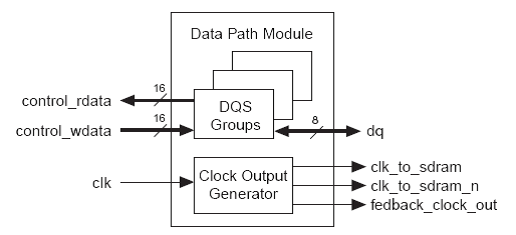
\includegraphics{sample1.png}\\
  \caption{算法流程图}\label{fig:algo}
\end{figure}

图 \ref{fig:algo} 展示了算法流程。

\begin{figure}[!ht]
  \centering
  % Requires \usepackage{graphicx}
  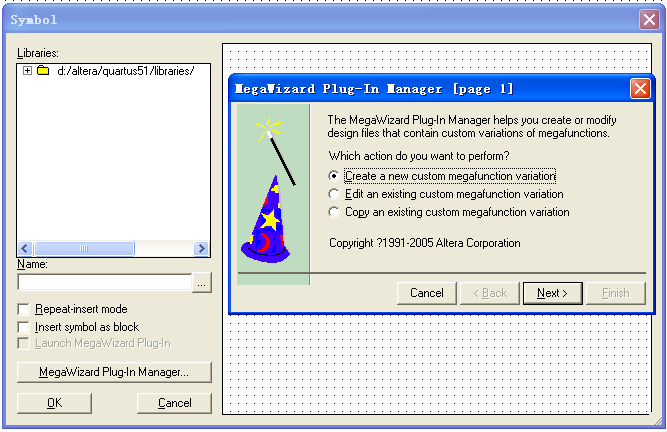
\includegraphics[scale=0.5]{sample2.png}\\
  \caption{算法流程图}\label{fig:ui}
\end{figure}

图 \ref{fig:ui} 展示了操作界面。

\subsection{注释}
注释是对论文中特定名词或新名词的注解。注释可用页末注或篇末注的一种。选择页末注的应在注释与正文之间加细线分隔,线宽度为1磅,线的长度不应超过纸张的三分之一宽度。同一页类列出多个注释的,应根据注释的先后顺序编排序号。字体为宋体5号,注释序号以“\circled{1}、\circled{2}”等数字形式标示在被注释词条的右上角。页末或篇末注释条目的序号应按照“\circled{1}、\circled{2}”等数字形式与被注释词条保持一致。示例我需要注释啊\footnote{我是解释注释的}。



\subsection{参考文献}
参考文献的著录应符合国家标准,参考文献的序号左顶格,并用数字加方括号表示,与正文中的引文标示一致,如[1],[2]……。每一条参考文献著录均以“.”结束。具体各类参考文献的编排格式
这里需要注释\footnote{我是脚注}。
\subsection{附录}
论文附录依次用大写字母“附录A、附录B、附录C……”表示,附录内的分级序号可采用“附A1、附A1.1、附A1.1.1”等表示,图、表、公式均依此类推为“图A1、表A1、式(A1)”等。

\subsection{印刷与装订顺序}
毕业论文应按以下顺序装订:封面→学术声明→中文摘要→英文摘要→目录→正文→参考文献→致谢→附录

\section{研究背景}
介绍所要解决问题的背景、选题的意义

\section{研究目标}

介绍所要解决的问题这里需要注释\footnote{我是脚注}。
\section{论文结果}

介绍论文的结果、取得的成果
\section{论文结构}
介绍论文的组织结构
这里需要注释\footnote{我是脚注}。
%%%%%=== background ===%%%%%
\chapter{相关技术}

可以分节介绍所要用到的相关知识、工具。
\section{背景知识}
相关知识

\section{工具}
相关工具
这里需要注释\footnote{我是脚注}。
%%%%%=== work ===%%%%%
\chapter{核心内容}
主要介绍论文研究的核心内容
\section{问题定义}
问题的详细定义与描述
这里需要注释\footnote{我是脚注}。
\section{数据}
用到的主要数据结构定义或硬件(如芯片)的有关说明

\subsection{采样方式}
设计数据采集方式
\subsection{数据选择}
选择符合标准的数据

\section{方法}
解决方案的总体描述

\subsection{数据处理}
如何处理数据,详细方法

\subsection{中间结果分析}
分析中间结果

\section{总结}
解决方案的详细介绍


%%%%%=== result ===%%%%%
\chapter{结果分析}
如果提出新的算法,需要证明算法的正确性、分析复杂性(不能证明时,至少是说明)。给出实验/实现结果(可以用图、表、定理),并对结果给出必要的分析与说明。论文应该有设计和实现的过程及相关结果,理论探索论文,应有模拟实验结果。
\section{小标题}
实验结果
\section{小标题}
误差分析

%%%%%=== conclusion ===%%%%%
\chapter{结论与展望}
包括结论与展望
\section{结论}
结论是毕业论文的总结,是整篇论文的归宿。应精炼、准确、完整。着重阐述自己的创造性成果及其在本研究领域中的意义、作用,还可进一步提出需要讨论的问题和建议。
\section{前景}
展望未来,表明对所做的工作有进一步推动的愿望。

%%%%%=== 参考文献 ===%%%%%
\clearpage\phantomsection
\addcontentsline{toc}{chapter}{参考文献}
\begin{thebibliography}{00}

  \bibitem{J} 作者. 文章题目[J]. 期刊名, 出版年份,卷号(期数):起止页码.

  \bibitem{M} 作者. 书名 [M]. 版次. 出版地:出版单位,出版年份:起止页码.

  \bibitem{A} 作者. 文章题目[A].主编.论文集名[C], 出版地:出版单位,出版年份:起止页码.

  \bibitem{D} 作者. 论文题目[D].保存地:保存单位,年份.

  \bibitem{R} 报告者. 报告题目[R].报告地:报告会主办单位,报告年份.

  \bibitem{P} 专利所有者. 专利名称:专利国别,专利号[P].发布日期.

  \bibitem{S} 标准代号. 标准名称[S].出版地:出版单位,出版年份.

  \bibitem{N} 作者. 文章题目[N].报纸名,出版日期(版次).

  \bibitem{O} 作者.文献题目[电子文献及载体类型标识].电子文献的可获取地址,引用日期.


\end{thebibliography}
\par
电子参考文献建议标识:
\begin{itemize}
  \item [DB/OL]——联机网上数据库(database online)
  \item [DB/MT]——磁带数据库(database on magnetic tape)
  \item [M/CD] ——光盘图书(monograph on CD-ROM)
  \item [CP/DK]——磁盘软件(computer program on disk)
  \item [J/OL] ——网上期刊(serial online)
  \item [EB/OL]——网上电子公告(electronic bulletin board online)
\end{itemize}


\addcontentsline{toc}{chapter}{致谢}
\chapter*{致谢}

表达作者对完成论文和学业提供帮助的老师、同学、领导、同事及亲属的感激之情。

\clearpage
\appendix

\chapter{程序}
对于一些不宜放在正文中的重要支撑材料,可编入毕业论文的附录中。包括某些重要的原始数据、详细数学推导、程序全文及其说明、复杂的图表、设计图纸等一系列需要补充提供的说明材料。
\section{定位}
测试程序
\subsection{小节}
这是个小节
\section{导航}
运行程序

\chapter{数据}
\section{实例}
数据示例

\end{document} 